\section{Crystal and Band Structure of Bi$_2$Te$_2$Se}
\label{sec:bts:bts-band}

Bi$_2$Te$_2$Se's crystal structure is similar to Bi$_2$Te$_3$, with a tetradymite structure and a rhombohedral unit cell. Its space group is $R\bar{3}m$. As shown in Fig. \ref{BTS_structure}A, compared with Bi$_2$Te$_3$, the Te layer between two Bi layers in Bi$_2$Te$_2$Se is replaced by one Se layer~\cite{Ando10}. Since the Bi-Se bonds are stronger than the Bi-Te bonds, the Bi atoms are more likely to stay on their sites than to exchange the sites with Te atoms. Thus such a structure may reduce p-type carriers caused by Bi-Te anti-sites. Besides, compared with Bi$_2$Se$_3$, there are no two adjacent Se layers in Bi$_2$Te$_2$Se. The lack of Se-Se bonds in could also reduce Se vacancies as the Se-Se bonds are not strong and may produce Se vacancies. As a result, the crystal structure of Bi$_2$Te$_2$Se may reduce both the n-type and p-type carriers intrinsically. 

\begin{figure}[!htbp]
  \begin{center}            
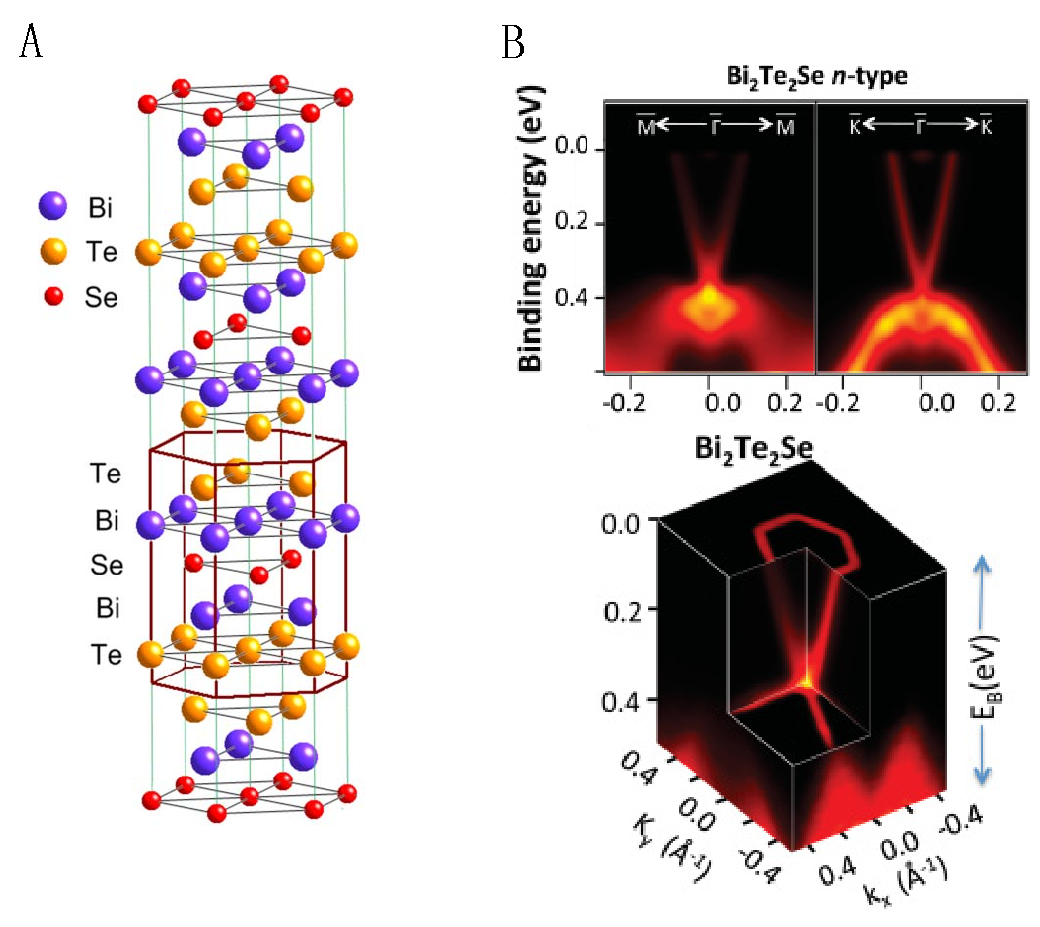
\includegraphics[width=0.9\linewidth]{ch-bts/figures/BTS_structure.pdf} 
\caption{\label{BTS_structure} (Color online) 
The crystal structure and band structure of Bi$_2$Te$_2$Se. (A) The crystal structure of Bi$_2$Te$_2$Se is similar to that of Bi$_2$Te$_3$ with the Te layer between two Bi layers replaced by one Se layer~\cite{Ando10}. (B) The ARPES experiment shows that Bi$_2$Te$_2$Se has a band structure similar to Bi$_2$Te$_3$~\cite{BTS_ARPES}. The band gap is also as large as approximately 0.3 eV, while the surface Dirac point is immersed in the valence band as well.
} 
  \end{center}
\end{figure}

Similar to Bi$_2$Se$_3$ and Bi$_2$Te$_3$, Bi$_2$Te$_2$Se's strong spin-orbital coupling inverts its bulk bands as well. Fig. \ref{BTS_structure}B is the ARPES data on Bi$_2$Te$_2$Se by Hasan's group~\cite{BTS_ARPES}. It demonstrates a clear bulk band gap of approximately 0.3 eV. The V-shape state in Fig. \ref{BTS_structure}B is the spin-polarized single surface Dirac cone. The Dirac point of the surface states is buried in the valence band, as in the case of Bi$_2$Te$_3$.